\documentclass{article}
\usepackage{xeCJK}
\usepackage{cite}
\usepackage{booktabs}
\usepackage{amsmath,amsfonts,amsthm,amssymb}
\usepackage{setspace}
\usepackage{fancyhdr}
\usepackage{lastpage}
\usepackage{extramarks}
\usepackage{chngpage}
\usepackage{soul,color}
\usepackage{graphicx,float,wrapfig}
\usepackage[colorlinks,linkcolor=blue]{hyperref}

\topmargin=-0.85in      %
\evensidemargin=0in     %
\oddsidemargin=0in      %
\textwidth=6.5in        %
\textheight=9.0in       %
\headsep=0.25in         %


\title{\bf Proposal for Introduction to Data Science}
\author{Chen Ying, Liu Guoding, Mao Haining, Zhu Simo}
\date{December,2019}
\begin{document}

\maketitle

\section{Problem background}
Text data is around us everywhere, and how to deal with those words, sentences or passages has long been a hot topic for natural language processing fields. All contexts contain two kinds of information: semantic information and syntactic information. Study of the former can leads to judgement for each single word and phrase, and study of the latter focus more on the organization of texts. Above all, the key problem is the way to extract features from the text.
\\ \hspace*{\fill} \\
With the rapid development and popularization of social media services, rumors are spreading with unprecedented rapidity and have a tremendous impact on human society. Meanwhile, the development of artificial intelligence technologies provides a promising approach for social media platform to automatically detect rumors. Under that situation, we hope to set up a model to distinguish those rumors from normal ones with only contents or make predictions based on all comments when users forward the message.
\\ \hspace*{\fill} \\
We are curious about how the sequential and contextual information influence the authenticity of a given context, how different representing methods and classification models performs on this classification problem. How the propagation process of rumor helps the detection, and what characteristic comments of the message and time series information have. If the dataset is unbalanced, how does the scarcity act on the training process of the dataset and its performance on different evaluation indicator. If possible, we hope our primary features can be explanatory for deeper analysis of rumor. 

\section{Dataset Specification}
This data is the Chinese rumor data captured from sina weibo false information reporting platform, which is divided into two parts. The first data set contains a total of 31,669 rumors from September 4, 2009 solstice June 12, 2017 with the title content of the rumor reported, the name of the whistleblower's microblog, the link of the whistleblower's microblog, the name of the rumorist's microblog, the link of the rumorist's microblog, the rumor content, the number of visits to the rumor, the censorship result of the rumor, and the time when the rumor was reported.
\cite{liu2015rumors}
\\ \hspace*{\fill} \\
\{"rumorCode":"K1CaN8wJg7a0e",\\\ "title":"@无处安放大脸喵 举报@小小小小小吖莲 不实信息",\\\ "informerName":"无处安放大脸喵",\\\ "informerUrl":"http://weibo.com/u/5198423515",\\\ "rumormongerName":"小小小小小吖莲",\\\ "rumormongerUrl":"http://weibo.com/u/5246061392",\\\ "rumorText":":上海城管暴力执法,同学的舅妈被打死了,报警了可是公安只说等回复,求给一个公道,城管为什么可以这么嚣张?求解释? http://t.cn/RUUefZa",\\\ "visitTimes":4,\\\ "result":"此微博称“上海市颛桥城管打死人了”不实,据@警民直通车-闵行通报:市容管理人员葛路某准备骑电瓶车离开现场,被路边设摊人员黄某阻拦。黄某儿子葛树某驾驶一辆蓝色……",\\\ "publishTime":"2016-06-13 16:18"\}
\\ \hspace*{\fill} \\
The second part of the dataset (CED\_Dataset) contains the forwarding and comment information related to the original microblog, including 1538 rumors and 1849 non-rumors. This data set is divided into original weibo posts and their forwarding/commenting content. The non-rumor repost and rumor repost, respectively contain the corresponding forwarding and comment information of the non-rumor and rumor original. (this dataset does not distinguish between comments and forwarding.) In this dataset, each original article, comment or comment is in json format.
\cite{song2018ced}

\begin{figure}[ht]
	\centering  
	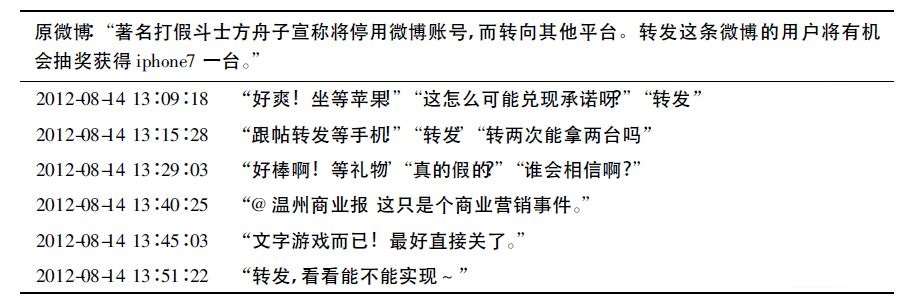
\includegraphics[width=0.8\linewidth]{dataset.jpg}  
\end{figure}
The dataset can be download from the website: \href{https://github.com/thunlp/Chinese_Rumor_Dataset}{Chinese\_Rumor\_Dataset}

\section{Preliminary Technical Solution}
Since text data is unstructured, some preprocessing, such as removing punctuation marks, special characters, and urls, is usually required before analysis. Li offers a preprocessing method for unnormalized words.\cite{litwitter}
\\ \hspace*{\fill} \\
Early automatic rumor detection method was to design classification features based on relevant information of suspected rumors, we hope the feature can be extracted by my model itself. Several encoding methods for texts have been proposed: Bag of Words(BOW), Word2Vec, FastText, GloVe, etc. There are also various language models that can fulfill our goal: Transformer, CNN(convolutional neural network), RNN(Recurrent Neural Network), and so on. Times series information can also apply some well-performed feature extractor.
\\ \hspace*{\fill} \\
We want to find out the characteristic for different model and then choose the best suitable model in later research, if possible, each model will be analyzed.

\section{Evaluation Metrics}
Since the number of samples in each category of corpus is relatively balanced, we use accuracy as the evaluation index:
\[Accuracy=T/N\]
We are also interested in the influence of scarcity, if possible, we hope to train our model on randomly-split dataset, and analyze its impact.

\bibliographystyle{plain}
\bibliography{ref} 
\end{document}
